\section{Durchführung}
\label{sec:Durchführung}

\begin{figure}[H]
  \centering
  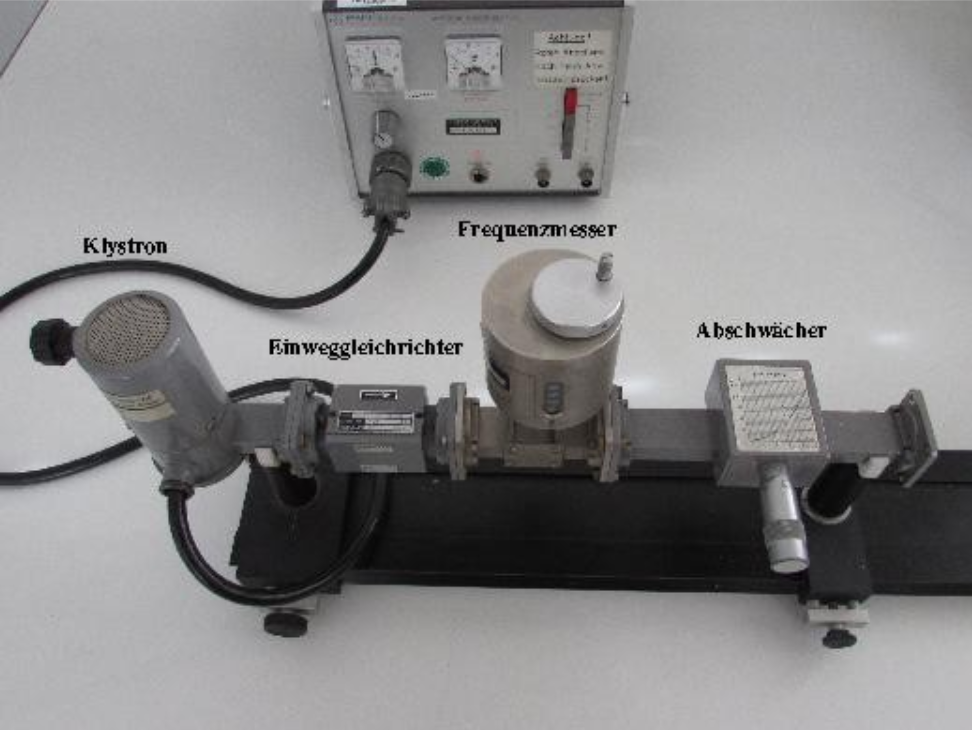
\includegraphics[height=10cm]{Grundaufbau.PNG}
  \caption{Grundlegender Aufbau des Versuchs. \cite{sample}}
  \label{fig:aufbau}
\end{figure}

Für alle der im Folgenden beschriebenen Versuchsteile wird der gleiche Grundaufbau
entsprechend Abbildung \ref{fig:aufbau} verwendet. Ein Reflexklystron wird über ein
Speisegerät mit Spannung versorgt. Dieses erzeugt, wie in der Theorie beschrieben,
Mikrowellen, die dann in den daran angeschlossenen Hohlleiter geführt werden.
Anschließend durchlaufen sie einen Einweggleichrichter sowie einen Frequenzmesser.
Letzterer besteht aus einem koaxialen Resonator, dessen Resonanzfrequenz über
ein rotierbares Rad geändert werden kann. Wird er nun genau mit seiner Resonanzfrequenz
angeregt und somit zur Resonanz gebracht, so entzieht der er dem Hohlleiter
einen Teil seiner Leistung. Dies kann wiederum später auf einem Anzeigeinstrument
sichtbar gemacht werden.
Hinter dem Frequenzmesser liegt dann noch ein Abschwächer. Bei dem Dämpfungselement
handelt es sich um eine Widerstandsfolie, die durch das Verstellen einer Schraube
parallel zum elektrischen Feld verschoben werden kann. Je nach Lage der Folie im
Hohlleiter tritt eine unterschiedliche Dämpfung ein. Man erhält gerade eine maximale
Dämpfung, wenn die Folie in der Mitte des Hohlleiters liegt.

\begin{figure}[H]
  \centering
  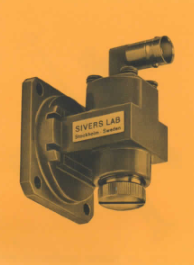
\includegraphics[height=6cm]{Diode.PNG}
  \caption{Abbildung des Diodendetektors. \cite{sample1}}
  \label{fig:diode}
\end{figure}

Im ersten Versuchsteil wird das Dämpfungsglied auf 30 dB eingestellt und
am Ende des oben beschriebenen Grundaufbaus lediglich eine Diode (Abbildung \ref{fig:diode}) angebaut.
Diese wird dann über ein Kabel an den Y-Kanal eines
Oszilloskops angeschlossen. Auf den X-Kanal des Oszilloskops wird ebenfalls durch
das Speisegerät eine Spannung gegeben, welche jedoch hier mit einer entsprechenden
50 kHz Referenzfrequenz moduliert wird. So können dann die einzelnen Schwingungsmoden
des Klystrons (Abbildung \ref{fig:mode}) auf dem Oszilloskop sichtbar gemacht werden. Die Amplitude und Lage
von drei dieser Moden wird vermessen. Zudem wird auch die Frequenz an der
Stelle derer Maxima gemessen.

\begin{figure}[H]
  \centering
  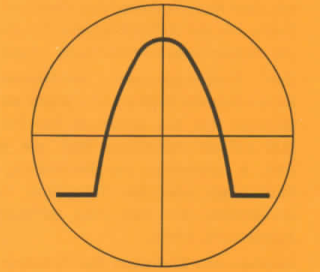
\includegraphics[height=5cm]{Mode.PNG}
  \caption{Eine Modenkurve. \cite{sample1}}
  \label{fig:mode}
\end{figure}

Im zweiten Versuchsteil wird die oben genannte feste Diode durch eine parallel
zum Hohlleiter bewegliche Diode, den sogenannten Stehwellen-Detektor (Abbildung \ref{fig:stehwellendetektor}), ausgetauscht. Dieser wird dann an ein SWR-Meter angeschlossenen.
Dahinter wird dann auch noch ein Gleitschraubentransformator und ein Kurzschluss angebaut.
Der Gleitschraubentransformator besteht aus einem Stück Hohlleiter, in welches über eine Drehschraube ein einfacher
Metallstift hinein gedreht werden kann. Dieser findet jedoch erst im folgenden Versuchsteil
Verwendung und wird hier dementsprechend komplett hinaus gedreht. Der Kurzschluss
dient zur vollständigen Reflexion der einlaufenden Mikrowellen. Durch ihn kann
im Inneren des Hohlleiters also ein Stehwellenfeld erzeugt werden. Mit Hilfe der
verschiebbaren Sonde werden dann lediglich die Positionen der einzelnen Minima
im Stehwellenfeld gemessen, indem der Ausschlag am SWR-Meter bei Variation der
Sondenposition beobachtet wird.

\begin{figure}[H]
  \centering
  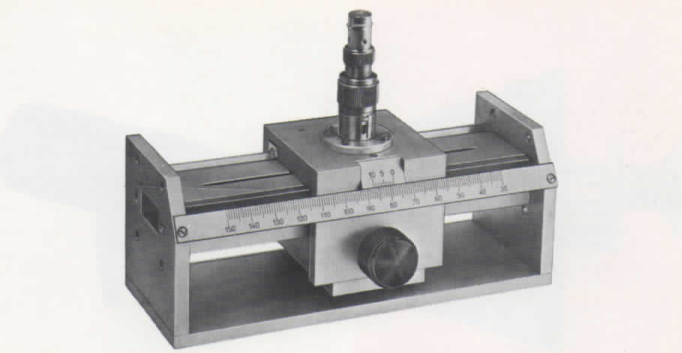
\includegraphics[height=6cm]{Stehwellendetektor.PNG}
  \caption{Der Stehwellendetektor. \cite{sample1}}
  \label{fig:stehwellendetektor}
\end{figure}

Anschließend soll die Dämpfung bestimmt werden. Diese wird ebenfalls einfach am
SWR-Meter für unterschiedliche Einstellungen des Dämpfungsgliedes abgelesen.

Im vierten und letzten Versuchsteil soll dann noch das Stehwellenverähltnis (SWR) bestimmt werden.
Dies kann über drei unterschiedliche Methoden geschehen.
Dazu wird in der Versuchsanordnung lediglich der Kurzschluss durch einen Abschluss ersetzt.
Dieser reflektiert die einlaufenden Wellen nicht, sondern er absorbiert sie vollständig.
Die erste Methode ist die "direkte Methode". Dabei wird das SWR direkt mit der
Sonde bestimmt. Diese wird zu beginn so positioniert, dass sie sich in einem
Maximum des Stehwellenfelds befindet. Anschließend wird die Verstärkung des SWR-Meters
so variiert, dass dieses einen Wert von 1,0 anzeigt. Dann wird die Sonde in ein Minimum
verschoben. Der Wert, den das SWR-Meter dann anzeigt, ist das gesuchte Stehwellenverhältnis.
Diese Messung wird ebenfalls für andere Einstellungen des Gleitschraubentransformators
(0 mm, 3 mm, 5 mm, 7 mm) wiederholt.

Die zweite Methode ist die 3dB-Methode. Dabei wird die Sonde zuerst in ein Minimum
des Stehwellenfeldes verschoben. Die Verstärkung des SWR-Meters wird dann so eingestellt,
dass sich eine Anzeige von 3 dB ergibt. Anschließend wird die Sonde nach links verschoben,
bis sich am SWR-Meter ein maximaler Ausschlag (0 dB) ergibt. Das Gleiche wird auch für
eine Verschiebung nach rechts getan. Aus den sich dabei jeweils einstellenden Werten am SWR-Meter
lässt sich das SWR berechnen. Auch diese Messung wird für jede einzelne der oben genannten Einstellungen
des Gleitschraubentransformators durchgeführt.

Die dritte Methode ist die Abschwächer-Methode. Die Sonde wird dabei wieder in einem
Minimum positioniert, um den sich dabei einstellenden Wert am SWR-Meter zu ermitteln.
Das Dämpfungsglied wird hier nun auf einen Wert von 20 dB eingestellt.
Anschließend wird die Sonde in ein Maximum verschoben. Dann wird das Dämpfungsglied
so umgestellt, dass sich in diesem Maximum der gleiche Wert wie zuvor beim Minimum
am SWR-Meter ergibt. Aus der Änderung der Dämpfung lässt sich dann das Stehwellenverhältnis
ermitteln.
